\section{Inverse Texture Synthesis}
Another algorithm for summarizing images is the \textit{inverse texture synthesis} found by \textsc{Wei, Han, Zhou, Bao, Guo} and \textsc{Shum}.\\
It works similar to bidirectional similarity (see section 2) by comparing for completeness and coherence. Those steps only have different names (forward M-step and inverse M-step) and the algorithm does not use gradual resizing instead the target images changes continously. \\
Inverse texture synthesis brings a user-controlleable feature with it: control maps. So we will first learn about control maps and then introduce the technical details of the algorithm.

\subsection{Control maps}
As mentioned before control maps are a big feature in inverse texture synthesis not only because they are user-controllable. Technically they are an additional layer for computation to manipulate how the final texture will look like similar to importance weights of bidirectional similarity (section 2.3.3).\\
Figure \ref{fig:Control maps} shows an example for control maps. As you can see the control maps 'controls' where the brown spots are located on the final texture. The non-black parts work like a mask to show a desired percentage of the brown spots where white means 100\% brown.\\
If we would change the white parts of the control map, the brown spots on he texture would change too.\\
User can define their own control maps to achieve different textures like painting dirt on a mesh\footnotemark  of a vase. 

\footnotetext{A \textit{mesh} is a collection of polygons in 3D computer graphics representing a 3D object.}

\begin{figure}[h]
\centering
\includegraphics[scale=0.9]{img/controlmaps}
\caption[Control maps]{On the left a texture, on the right the control map for the texture.\\ Images from \cite{its}.}
\label{fig:Control maps}
\end{figure}


\subsection{Algorithm}
The algorithm of inverse texture synthesis starts by filling the compactation with random pixels from the original image. Not only the color information from the pixel will be copied also the original location of it so it can be compared to its neighbors in the original image.\\
Like the bidirectional similarity it is a two-way comparison of patches by finding the most similar ones (section 2.1). The check for coherence is called \textit{forward M-step} and the check for completeness is called \textit{inverse M-step}.\\
The last step of the algorithm is called \textit{w E-step} where the result is manipulated by an \textit{orientation field}.

\begin{figure}[h]
\centering
\includegraphics[scale=0.75]{img/its-algo}
\caption[Inverse texture synthesis algortihm]{This figure shows different steps of the algorithm. (a) shows the z E-step and forward M-step. (b) illustrates the inverse M-step.}
\label{fig:Inverse texture synthesis algortihm}
\end{figure}

\subsubsection{z E-step}
After initializing the compactation \textit{T} with random pixels from the original image \textit{S}, the algorithm selects a pixel in \textit{T}.
Figure \ref{fig:Inverse texture synthesis algortihm} (a) shows the selected pixel $0$. Pixel $0$ has neighbors ${1,2,3,4}$ which do have a origin in the original image \textit{S}.\\
The origin was also copied when initializing the compactation with random pixels. The neighbors ${1,2,3,4}$  also have neighbors in the original image - in this case those are ${5,6,7,8}$.\\
From the neighbors ${5,6,7,8}$ the algorithm can now calculate a median color for pixel $0$.

\subsubsection{Forward M-step}
The forward M-step is similar to coherence check in bidirectional similarity. This step does not need any additional computation, for a patch $Q$ in $T$ containing pixel $q$ it just looks for a best matching patch $P$ in $S$.\\
In Figure \ref{fig:Inverse texture synthesis algortihm} (a) the forward M-step could be finding the best matching pixel from ${5,6,7,8}$ to pixel $0$. This is a constant time operation and not applicable to the inverse M-step. 

\subsubsection{Inverse M-step}
\subsubsection{w E-step}
In the last step, called \textit{w E-step}, the algorithm uses an orientation field to optimize the result of compactation. It works like and additional layer of information.

\begin{figure}[h]
\centering
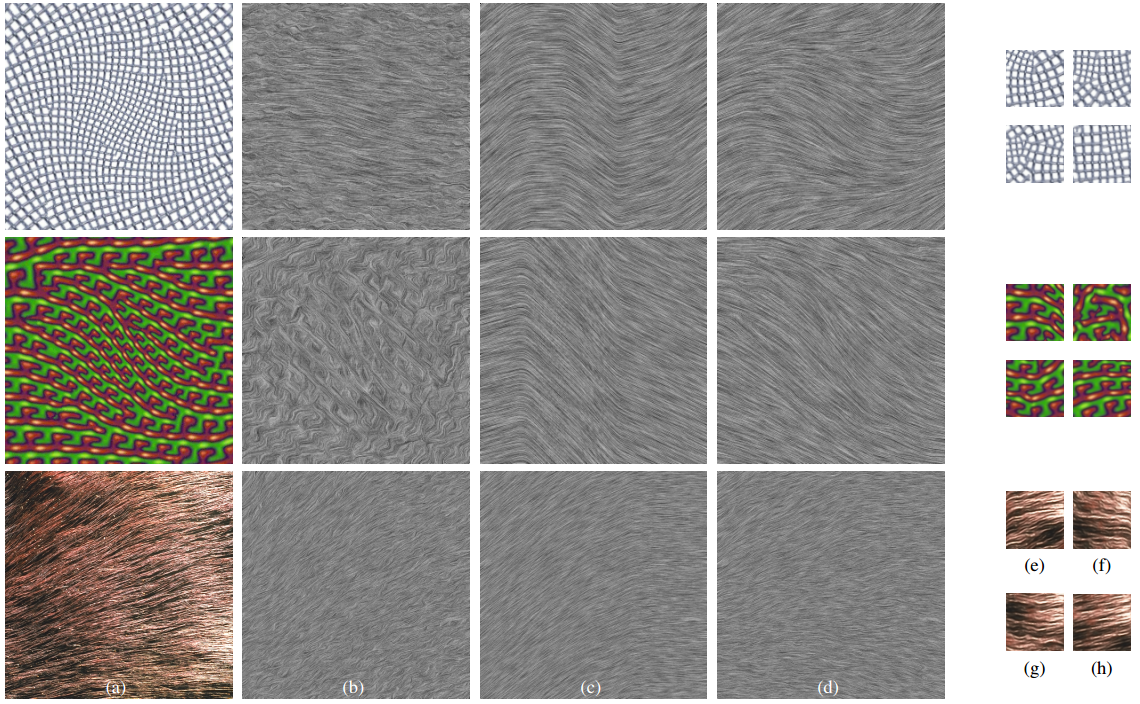
\includegraphics[scale=0.4]{img/orientationfield}
\caption[Orientation field]{This figure shows within each row different orientation fields. (a) is the orignal texture with uniform x-y-orientation. (b) shows the orientation fields from \cite{paris}. (c) shows orientation fields via manual specification followed by interpolation. And (d) is the orientation field from \cite{its} based on (c).\\ Images from \cite{its}.}
\label{fig:Orientation field}
\end{figure}


\subsection{Example}
\subsection{Performance and limitations}